\documentclass[12pt]{article}
\usepackage{amsmath}
\usepackage{amsthm}
\usepackage{amsfonts}
\usepackage{graphicx}
\usepackage{epstopdf}
\usepackage{float}
\usepackage{fancyhdr}
\usepackage{hyperref}
\usepackage{subcaption}
\usepackage{pdfpages}
\usepackage{algpseudocode}
\usepackage{framed}
\usepackage{amssymb}



\makeatletter
\renewcommand\@biblabel[1]{}
\renewenvironment{thebibliography}[1]
     {\section*{\refname}%
      \@mkboth{\MakeUppercase\refname}{\MakeUppercase\refname}%
      \list{}%
           {\leftmargin0pt
            \@openbib@code
            \usecounter{enumiv}}%
      \sloppy
      \clubpenalty4000
      \@clubpenalty \clubpenalty
      \widowpenalty4000%
      \sfcode`\.\@m}
     {\def\@noitemerr
       {\@latex@warning{Empty `thebibliography' environment}}%
      \endlist}
\makeatother

\theoremstyle{definition}
\allowdisplaybreaks
\fancyhf{}


\DeclareMathOperator*{\Max}{Max}
\DeclareMathOperator*{\Min}{Min}
\setlength{\parindent}{0cm}



\begin{document}

\title{Loss Distributions: Computational Efficiency in an Extended Framework}
\date{}
\author{Daniel H. Stahl}

\maketitle
Word Count: 3491
\\
\\
Figures and Tables: 8
\\
\\
Acknowledgments: The author reports no conflicts of interest.  The author alone is responsible for the content and writing of the paper.
\newpage
 \begin{abstract}
Credit risk models are difficult to implement in an actionable form.  While near real-time results are required for pricing credits, making origination decisions, and optimizing portfolio allocation, the complexity of credit models (which are often employed on portfolios spanning millions of exposures) typically requires either expensive Monte Carlo simulations or the imposition of inflexible assumptions to compute the portfolio loss distribution.  The contribution of this paper to the credit risk literature is twofold: Credit Suisse's Credit Risk \(^+\) framework is significantly generalized, and an algorithm from the option pricing literature is introduced to retain precision and speed for the computation of the loss distribution even for very large portfolios.  This generalization allows for time-dependent portfolios, fully accounts for granularity and concentration within the credit portfolio, and does not rely on assumptions of asymptotically large credit portfolios.  The algorithm allows even a standard laptop to precisely compute an entire bank's loss distribution.
\\
\\
Core Results:
\begin{enumerate}
\item The model uses a stochastic process as the state variable yet retains tractability.
\item The model integrates liquidity risk into the credit loss distribution.
\item Algorithm from the option pricing literature is leveraged for efficient computation.

\end{enumerate}

Keywords: Credit Risk \(^+\); Mixture Models; Credit Portfolio; Fourier Inversion; Loss Distribution
\end{abstract}


\newpage
\section{Introduction}
It is a common credit risk modeling technique to introduce random variables that jointly affect the probability of default of distinct creditors.  This class of models is termed ``mixture'' models due to the ``mixing'' of the default probability with other random variables.  Categories of mixture models differ in the specification of the random variables that effect the probability of default.  Merton (1974) created one of the first mixture models for estimating the probability of default for a single firm by defining default as the realization of negative equity at the some fixed time horizon.  The firm's assets are modeled by a diffusion process which serves as the ``mixing'' random variable.  Since default is determined by an underlying economic factor, models for firm's assets are dubbed ``factor'' or ``structural'' models.  Black and Cox (1976) extend Merton by defining default as the first occurrence of negative equity at any time prior to the time horizon.  Both of these models feature endogenous default.  ``Intensity'' or ``Reduced form'' models are another strand of research that treats the cause of default as exogenous.  In these models the default intensity (which, for small probabilities of default, is roughly the probability of default) follows a latent stochastic process.  Jarrow and Turnbull (1995) pioneered this approach while Duffie (2005) provides a detailed overview.    
\\
\\
Merton,  Black and Cox, and Jarrow and Turnbull focus on modeling individual defaults.  For many banks the entire loss distribution of credit portfolios is of more concern than pricing individual defaults.  Early research in modeling the loss distribution extended Merton's model.  Vasicek (1987), (1997) uses the Merton framework with each firm's asset returns following correlated diffusion processes.  He then channels the Capital Asset Pricing Model (CAPM) by reducing each firm's asset returns into an idiosyncratic and a systemic component.  The systemic component drives correlation between defaults.  In the idealized portfolio of homogeneous and atomic assets, the Vasicek model has an analytical solution for the portfolio density.  Extensions to Vasicek include multi-dimensional variations of systemic factors (Fok et al., 2014).  A common constraint on these models is that \(\lim_{n\to \infty} \sum_i ^n w_i ^2 \to 0\) where \(w_i\) is the relative exposure of asset \(i\).  For large banks, \(n\) is typically rather large and the assets are relatively diverse, satisfying the constraint.
\\
\\
Several industry models like J.P. Morgan's CreditMetrics (1997) use a more sophisticated version of Merton's model and compute the loss distribution via Monte Carlo techniques.  These models capture granularity and exposure concentrations, but are computationally expensive.  Credit Suisse First Boston's Credit Risk\(^+\) (2001) took a different approach to mixture models.  Instead of modeling underlying factors, the probability of default is a linear combination of the mixture variables.  The mixtures in these models lose the economic interpretation of a firm's assets, but gain considerable computational advantage.  However, the computational advantage is obtained by rounding exposures to integer values.  For a very diverse portfolio, this rounding leads to inaccurate modeling.  As default is exogenous, these models share conceptual similarities to reduced form models. 
\\
\\
A common trade-off with credit models is that either restrictive assumptions are introduced (eg an ``infinitely'' large portfolio in Vasicek's model or the rounding of exposures in the Credit Risk\(^+\) model), or the computation of the loss distribution is prohibitively time intensive.  The trade-off between complexity and accuracy is ubiquitous in any computational field, but is especially onerous when modeling credit portfolios where millions of data points must be analyzed while still providing timely results for business decisions. Indeed, computational convenience is essential for providing actionable information for a variety of banking decisions.  Loan committees need to make real-time decisions about the acceptability and pricing of the risk in the loans they approve.  Risk and capital committees make decisions for optimal portfolio allocations among loan asset classes, requiring efficient algorithms for the computation of marginal risks of individual assets and asset classes within the loan portfolio.  The contribution of this paper to the credit risk literature is twofold: the Credit Risk\(^+\) framework is significantly generalized to include liquidity risk, stochastic  exposures, and stochastic processes as mixture variables; and an algorithm from the option pricing literature is introduced to retain precision and speed for the computation of the loss distribution even for very large portfolios.  This framework allows for time-dependent portfolios, fully accounts for granularity and concentration within the portfolio, does not rely on asymptotically large portfolios, and can compute an entire bank's loss distribution on a standard laptop.  
\newpage
\section{Model Description}
\subsection{Assumptions}
There exists a portfolio of default-able assets.  The random variable describing this portfolio resides in a probability space \((\Omega, \mathcal{G}, \mathbb{P})\) with a filtration \(\mathcal{G}_t\) and a filtration \(\mathcal{F}_t \subset \mathcal{G}_t\) generated by \(W_t\), a single dimensional Brownian motion.  It is natural to consider the time period \(0\leq t \leq T < \infty\).  Let \(\tau_j,\,0<j\leq n\) be stopping times with respect to \(\mathcal{G}_t\) and let \(X_t ^ j\) be functions of \(\tau_j\) such that
\begin{equation}X_t ^ j=\begin{cases} l_j,\,\tau_j \in [t, T] \\ 0,\,\tau_j \not\in [t, T] \end{cases}\end{equation}
where \(l_j\) are mutually independent random variables.  Fixing \(T\), \(X_t ^j\) can be considered functions of \(\tau_j\) and hence are also random variables with the following distribution:
\begin{equation}\begin{cases} l_j,\, \mathbb{P}(\tau_j \in [t, T]|\mathcal{G}_t) \\ 0,\,1-\mathbb{P}(\tau_j \in [t, T] | \mathcal{G}_t)\end{cases}\end{equation}
\(X_t ^j\) has the interpretation of a return on a default-able asset.  Each \(X_t ^ j\) has a random exposure of \(l_j\) and a potential deterministic gain \(R_j\) at some time \(T\) if default has not occurred in \([0, T]\).  For simplicity, it is possible to consider the exposure \(l_j\) and a zero gain: once the loss distribution for the portfolio is computed, the entire distribution can be shifted by the sum of the expected returns to recover the profit and loss distribution.   The random variable describing the portfolio loss is denoted \(X_t=\sum_j X_t ^ j\).  From the definition of \(X_t ^j\), \(X_0 = 0\). 
\\
\\
The stopping times are distributed as follows:
\begin{enumerate}
\item
\( \mathbb{P}(\tau_j \in [0, T]|\mathcal{F}_T)=p_j Y_T \)
\item \(\tau_j\) and \(\tau_k\), \(j \neq k\), are independent conditioned on \(\mathcal{F}_T\)
\end{enumerate}
where each \(p_j\) is a constant and \(Y_t\) is a random process adapted to \(\mathcal{F}_t\).  \(\mathcal{F}_t\) represents the information available \emph{only} from the Brownian motion.  Knowledge of \(\mathcal{F}_t\) does not imply knowledge of the number of defaults in \([0,t]\), however knowledge of \(\mathcal{G}_t\) implies knowledge of all defaults in \([0, t]\).  \(\mathcal{F}_t\) is useful since conditioned on \(\mathcal{F}_t\) the defaults are mutually independent.  While the stopping times are independent conditioned on \(\mathcal{F}_T\), they are unconditionally dependent.  The unconditional dependence of the stopping times drives correlation between \(X_t ^ j\).  The rationale for using both \(\mathcal{F}_t\) and \(\mathcal{G}_t\) is perhaps best exemplified by considering a possible Monte Carlo estimation of the portfolio loss.  Generating a single path of \(Y_t\) (which is adapted to \(\mathcal{F}_t\)) yields information on the probability of default, but does not actually provide any information on the actual event of default.  Once a single path of \(Y_t\) is generated, the probability of default for each asset can be determined.  The process \(X_t\) can then be simulated using the probability of default generated by \(Y_t\). The process \(X_t\) is adapted to \(\mathcal{G}_t\), containing all the information in \(\mathcal{F}_t\) and the information for the actual defaults.  For a detailed discussion on the subject of filtrations in the context of defaults, see Appendix I in  Duffie (2001).    
\\
\\
Finally, 
\(Y_t\) is defined as \begin{equation} Y_t= \int_0 ^t Z_s ds\end{equation}
And \(Z_s\) solves the following stochastic differential equation (SDE):
\begin{equation} \label{sde} dZ_s=\alpha(1-Z_s)dt+\sigma \sqrt{Z_s} dW_t \end{equation}

\(Z_s\) is mean-reverting, non-negative, and has long run expected value of one (see appendix A.1).  Taking the differential of \(p_j Y_t\), \(d(p_j Y_t)=p_j Z_t dt\).  The long run instantaneous default rate is thus \(p_j dt\), permitting the interpretation of \(p_j\) as the long run default rate for \(X_t ^ j\) per unit time. \(Y_t\) can be interpreted as the effect the state of the economy has on the probability of default.
\\
\\
Technically, \(Y_t\) should be constrained to \([0, 1/p_k]\) where \(p_k\) is the large \(p_j\).  Without this constraint the probability of default can be greater than one.  However, relaxing this constraint allows the model to have a tractable solution.  In most practical applications the probability that any \(p_j Y_t\) is greater than one is too small to be consequential.  
\\
\\
In summary, the model contains a portfolio of \(n\) assets with the following features:
\begin{enumerate}
\item The assets have correlated defaults
\item The default correlation is driven by a latent \(\mathcal{F}_t\)-measurable variable \(Y_t\)
\item Each asset has a random but uncorrelated exposure \(l_j\)
\end{enumerate}

\subsection{Characteristic Function}
The characteristic function of a random variable is the Fourier transform of its density.  By the Fourier inversion theorem, taking the inverse Fourier transform of the Fourier transform recovers the density (Hewitt and Stromberg 1965).  The purpose of this section is to derive an analytic solution to the characteristic function of the portfolio loss distribution.  The characteristic function of \(X_t\) is
\begin{align}\phi_X (u, t) &=\mathbb{E}\left[e^{uiX_T}|\mathcal{G}_t\right]\\
&=\mathbb{E}\left[\mathbb{E} \left[ e^{uiX_{T}}|\mathcal{F}_T\right]|\mathcal{G}_t \right]\\
&=\mathbb{E}\left[  \prod_j \left(p_j (Y_T-Y_t) e^{ui l_j}+1-p_j(Y_T-Y_t)\right) |\mathcal{G}_t \right]\\
&=\mathbb{E}\left[  \prod_j \left(p_j (Y_T-Y_t) \mathbb{E}\left[e^{ui l_j}\right]+1-p_j(Y_T-Y_t)\right) |\mathcal{G}_t \right]\\
&=\mathbb{E}\left[  \prod_j \left(p_j (Y_T-Y_t) \phi_{l_j}+1-p_j(Y_T-Y_t)\right) |\mathcal{G}_t \right] \end{align}
Where \(\phi_{l_j}\) is the characteristic function of \(l_j\).  Note that if an asset has defaulted in \([0, t]\) then at time \(t\) it has value \(0\) with probability one.  The loss has already been realized and does not contribute to the loss distribution conditioned on \(\mathcal{G}_t\). 
\\
\\
For portfolios of reasonable size, the idiosyncratic nature of \(l_j\) diversifies away the risk of loss for each \(l_j\); causing the distribution to converge to the distribution where exposures are constant.  As shown in the appendix A.5, the contribution of the variance of \(l_j\) to the portfolio is proportional to \(n\) which is quickly dwarfed by a term that is proportional to \(n^2\).  However, there is no computational penalty for including a stochastic \(l_j\) and the advanced approach in Basel II encourages stochastic exposures (Basel Committee on Banking Supervision, 2006).  
\\
\\
If \(p_j (Y_T - Y_t)\) is small (as is typical of default models) then the following approximation holds by Taylor's theorem:
\begin{equation}\phi_X (u, t) \approx \mathbb{E}\left[ e^{\sum_j p_j(Y_T-Y_t) \left(\phi_{l_j}(u)-1\right)} | \mathcal{G}_t \right]\end{equation}
If the exposures are deterministic, the expression within the expectation is the characteristic function of a Poisson random variable and the Taylor approximation is equivalent to \(X_t ^ j\) following a Poisson distribution conditional on \(\mathcal{F}_T\) instead of a Bernoulli distribution.  As a Poisson random variable has sample space over the integers, the assumption that \(X_t ^j\) has a Poisson distribution implies that assets can have multiple ``defaults'', though the probability of more than one default is typically very small.  
\\
\\
Substituting \(p_j (Y_T - Y_t)=p_j\int_t ^T Z_s ds\) into the approximate characteristic function yields the following expression for \(\phi_X\):

\begin{align}\phi_X(u, t) &\approx \mathbb{E}\left[  e^{\int_t ^T Z_s ds\sum_j  p_j\left(\phi_{l_j}(u)-1\right)} |\mathcal{G}_t\right] \\
&\approx \mathbb{E}\left[  e^{v\int_t ^T Z_s ds} |\mathcal{G}_t \right] \end{align}
Where \(v=\sum_j  p_j \left(\phi_{l_j}(u)-1\right)\). Since \(v\) is deterministic, \(\mathbb{E}\left[  e^{v\int_t ^T Z_s ds} |\mathcal{G}_t \right]\) is the moment generating function of \(\int_t ^T Z_s ds\).  
\\
\\
The Feynman-Kac theorem states that for a suitable function \(h\) and diffusion process \(dB_t=\alpha(B_t, t)dt+\sigma(B_t, t)dW_t\) that
\(g(B_t, t)=\mathbb{E}\left[e^{\int_t ^T r(B_s)ds}h(B_T)|\mathcal{F}_t\right]\) satisfies the following partial differential equation (PDE) (Oksendal 2007):
\begin{equation}
\begin{cases} \frac{\partial g}{\partial t}+\frac{\partial g}{\partial b}\alpha(b, t)+\frac{\partial ^2 g}{2\partial b^2}\sigma^2 (b, t)+rg=0 \\
g(b, T)=h(b) \end{cases}
\end{equation}
Letting \(\phi(u, t) =\eta(z, t; v)=\mathbb{E}\left[  e^{v\int_t ^T Z_s ds} |\mathcal{G}_t \right]\) and leveraging the Feynman-Kac theorem,
\(\eta(z, t; v)\) satisfies

\begin{equation}
\begin{cases}\frac{\partial \eta}{\partial t}+\frac{\partial\eta}{\partial z}\alpha(1-z)+\frac{1}{2}\frac{\partial ^2 \eta}{\partial z^2} \sigma^2 z+vz=0 \\
\eta( z, T; v)=1\end{cases}
\end{equation}


Since this PDE is affine in \(z\), the solution has the form \(\eta(z, t; v)=e^{A(t, T)+C(t, T)z}\) (Duffie and Kan, 1996).  The set of SDE's which satisfy this affine form include the Vasicek (1977) and Cox, Ingersoll, and Ross (1985) interest rate models in one dimension, and the Heston (1993) model in two dimensions.  These ``affine'' models are computationally tractable even in higher dimensions since they only require solving a system of ordinary differential equations (ODEs) (Duffie and Kan, 1996).  In the case where \(z\) satisfies equation (\ref{sde}), the moment generating function has an analytical solution (Dufresne, 2001): 
\begin{equation} \label{eq1}\eta(z, t; v)= \left(\frac{e^{\alpha(T-t)/2}}{\beta}\right)^\frac{2\alpha}{\sigma^2} e^{\frac{vZ_t}{\gamma} \frac{2\text{sinh}(\gamma(T-t)/2)}{\beta}}\end{equation}
where \(\beta=\text{cosh}(\gamma(T-t)/2)+\frac{\alpha}{\gamma}\text{sinh}(\gamma(T-t)/2)\) and \(\gamma=\sqrt{\alpha^2-2v\sigma^2}\).  Substituting  \(v=\sum_j  p_j\left(\phi_{l_j}(u)-1\right)\) yields the analytical expression for \(\phi(u, t)\):
\begin{equation}
\phi(u, t)= \left(\frac{e^{\alpha(T-t)/2}}{\beta}\right)^\frac{2\alpha}{\sigma^2} e^{\frac{2 Z_t \left(\sum_j  p_j \left(\phi_{l_j}(u)-1\right)\right)\text{sinh}(\gamma(T-t)/2)}{\gamma \beta} }
\end{equation}
  Appendix A gives the analytical expressions for the moments of the loss distribution.

\subsection{Comparison to Intensity Models}

Intensity models often use option pricing theory to model the default of a bond (Duffie, 2005).  In particular, the probability of survival in \([0,\,t]\) is modeled as follows:
\begin{equation}1-\tilde{p}_t=\mathbb{\tilde{E}}\left[e^{-\int_0 ^t \lambda_s ds}\right]\end{equation}
The expectation is under the risk neutral measure and \(\lambda\) satisfies the following SDE:
\begin{equation}d\lambda_t=\alpha(b-\lambda_t)dt+\sigma\sqrt{\lambda} d\tilde{W}_t\end{equation}
This is a similar process to \(Z_t\) in equation (\ref{sde}).  Recall that the probability of default not occurring in the mixture model is, by the Poisson approximation, \(\mathbb{E}\left[e^{-p_jY_t}\right]\) where
\begin{equation} p_j Y_t= \int_0^t p_j Z_s ds \end{equation}
Letting \(\lambda_s=p_jZ_s\), it is clear that the two models coincide on the probability of default not occurring.  Thus the model proposed in this paper can be considered an extension of the intensity model  in much the same way that Vasicek extended Merton's model to compute the distribution of the entire portfolio.

\section{Liquidity Risk}
One of the major contributions of this paper is the introduction of semi-endogenous liquidity risk to credit portfolio modeling.  When credit losses start increasing, debt holders may start to become concerned and start pulling funding.  To meet these funding requirements, additional assets must be liquidated, likely at fire-sale prices.  While the probability of a liquidity crisis is non-zero at any level of credit loss, the probability of such a crisis increases as credit losses mount.  To retain an analytic expression for the characteristic function, the frequency of a liquidity crisis is modeled as a linear function of credit losses and the losses due to the liquidity crisis are assumed to be deterministic.  In addition, the liquidity crisis can only occur at \(T\) when the credit losses in \([0,\, T]\) have been made public.  Let \(C(t, T)\) be a random variable on \(\mathbb{R}^+\) that represents the potential dollar loss to the portfolio caused by fire-selling assets within the portfolio.  The distribution of \(C(t, T)\) is as follows:
\begin{equation}
C(t, T)=
\begin{cases}
\lambda(t, T),\, \text{with probability } q(X_T-X_t)+qX_t = q X_T \\
0,\,\text{with probability } 1-  q(X_T-X_t)-qX_t=1-qX_T
\end{cases}
\end{equation}
Here \(\lambda\) is the dollar loss in the event of a liquidity crisis and is a deterministic function of \(t\) and \(T\) while \(q\) is a non-negative constant that scales the dollar loss \(X_T\) so that the probability remains feasible.  For large loan portfolios, \(q\) should be rather small.  Letting \(t=0\) for simplicity, the total characteristic function is 
\begin{align}\mathbb{E}\left[e^{ui(X_T+C_T)}\right]&=\mathbb{E}\left[\mathbb{E}\left[e^{uiX_T} e^{uiC_T} | \mathcal{F}_T\right] \right]\\
&\approx \mathbb{E}\left[\mathbb{E}\left[ e^{uiX} e^{qX(e^{ui\lambda }-1)} |\mathcal{F}_T \right]\right]\\
&=\mathbb{E}\left[\mathbb{E}\left[ e^{\left(ui+q(e^{ui\lambda}-1)\right)X}| \mathcal{F}_T \right]\right]\\
&\approx \phi\left(u-iq(e^{ui\lambda }-1), 0\right) \end{align}
For \(\lambda=0\) or \(q=0\), the characteristic function reduces to equation (\ref{eq1}); as it should.  Figures (\ref{fig5}) and (\ref{fig6}) show the distributions of credit portfolios with various parameters.

\begin{figure}[htb]
\begin{framed}
Densities of the loss distribution of \(X_T\) with \(10,000\) assets.  Each asset has \(p=.03\) and exposure drawn from a Gamma\((10, 1000)\) distribution to ensure heterogeneous exposures. The densities are normalized to be a percentage of total exposure. \newline
\begin{minipage}[t]{.48\textwidth}
\centering
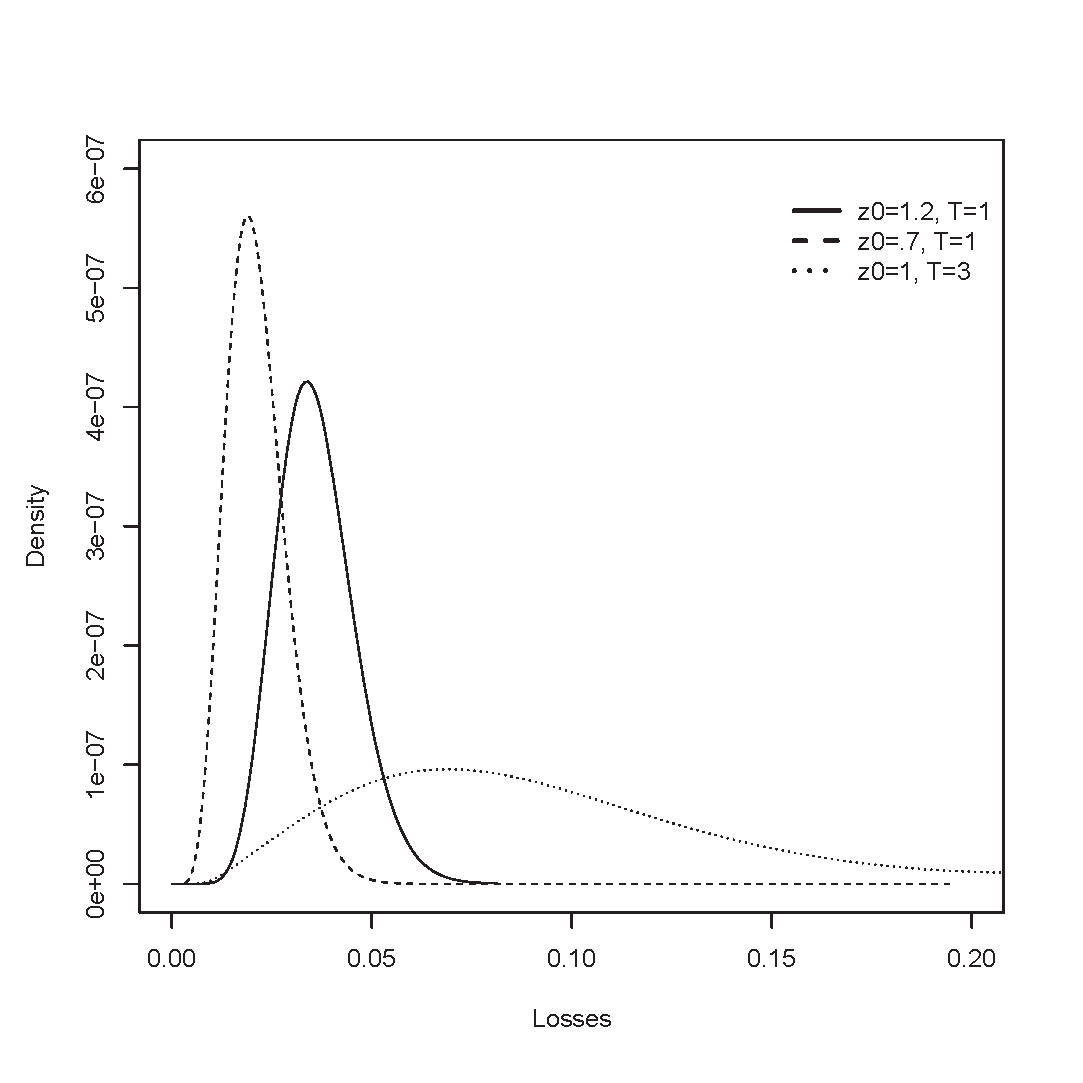
\includegraphics[width=1\textwidth]{Stahl6-9-2015Fig1}
\caption{\(\alpha=.3\), \(\sigma=.5\), \(\lambda=0\), \(q=0\).  \label{fig5}}
\end{minipage}\hfill
\begin{minipage}[t]{.48\textwidth}
\centering
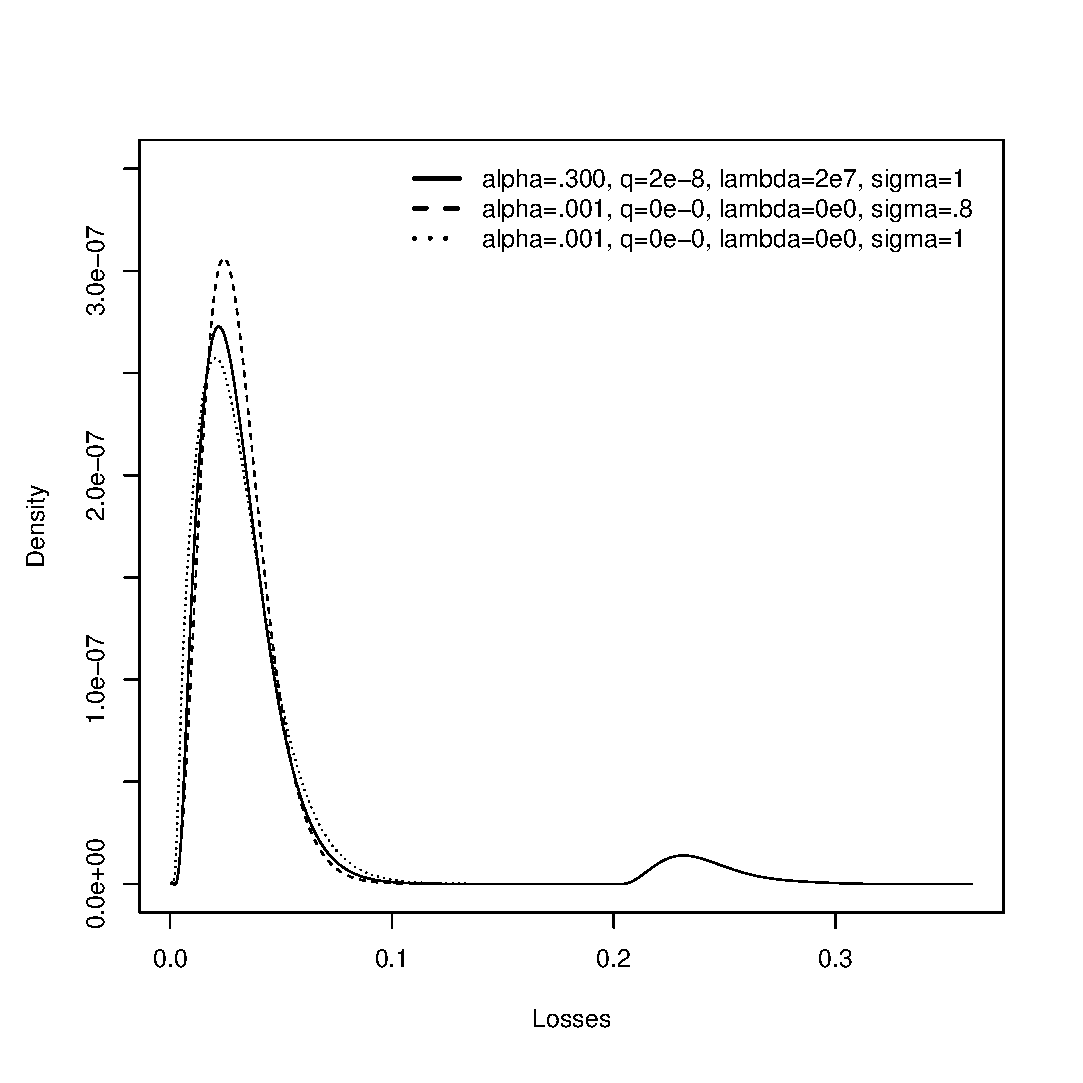
\includegraphics[width=1\textwidth]{Stahl6-9-2015Fig2}
\caption{\(z_0=1\), \(T=1\)  \label{fig6}}
\end{minipage}\hfill
\end{framed}
\end{figure}

\section{Numerical Inversion}
\subsection{Algorithms for Inversion}
With an analytic expression available for the characteristic function of \(X_T\), it is possible to invert the function to recover the loss distribution.  Letting \(f(x)\) be the density of \(X_T\), by the Fourier inversion theorem (Hewitt and Stromberg 1965), \begin{equation}f(x)=\frac{1}{2\pi}\int_{\mathbb{R}} e^{-iux} \phi(u, t) du \label{fourrier}\end{equation}
To solve this integral numerically, \(u\) and \(x\) must be discretized.  The loss distribution has support on \([0,\,x_{max}]\) where \(x_{max}\) is the sum of the total possible exposure on each asset.  \(x_{max}\) is an extreme upper bound on the possible losses in the portfolio, and it is often possible to truncate this range to provide superior accuracy for the same number of discrete intervals.  To obtain the numeric solution at each discrete point in \(x\), equation (\ref{fourrier}) must be numerically integrated for each discrete \(x\).  A naive implementation of this numeric integration has complexity \(O(mh)\) where \(m\) is the number of discrete steps in the \(u\) domain and \(h\) is the number of discrete steps in the \(x\) domain.  Using the  Fast Fourier Transform (FFT) reduces this complexity to \(O(m\mathrm{log}_2 (m))\) (Fang and Oosterlee 2008).  However, the FFT requires the same number of discrete steps in both the \(x\) and \(u\) domains.  Fang and Oosterlee (2008) use a cosine series expansion (COS) to invert the characteristic function instead of the FFT.  This expansion separates the discretization of \(u\) and \(x\) as well as providing exponential convergence for suitable functions.  For credit portfolio losses, the computationally difficult part is discretization of \(u\):  for each discrete \(u\) the entire characteristic function must be recomputed.  In a portfolio of \(n\) loans, the computation time for each discrete \(u\) is \(O(n)\). Hence the COS algorithm is perfectly suited for inverting characteristic functions since a fine mesh in \(x\) can be achieved while still using relatively few calls to the characteristic function.  The pseudo-code for the COS algorithm is presented in appendix B.
\\
\\
 Let \(m_{f}\) be the number of discrete steps in the FFT algorithm, let \(m_{c}\) be the number of steps in \(u\) for the COS algorithm, and \(h\) be the number of steps in \(x\) for the COS algorithm. The FFT algorithm for inverting the characteristic function has complexity \(O(m_{f}(n+\text{log}_2 (m_{f})))\) while the COS algorithm has complexity \(O(m_{c} (n +h))\).   As \(n\) grows, the COS algorithm converges to complexity \(O(nm_c)\) while the FFT algorithm, for fixed \(m_f\), has complexity \(O(n m_f )\). Thus the two algorithms, for \(m_f=m_c\), have similar complexity.  The similarity is confirmed in numerical tests in tables (\ref{table5}) and (\ref{table6}).


\subsection{Algorithm Results}
The moments of the distribution are known analytically and the first two are given in appendix A.  Using these moments is it possible to test the accuracy of each algorithm.  For the first and second moments, the expectation is numerically integrated over the approximate density from each of the two algorithms for a variety of parameters.  Letting \(M_i\) represent the \(i\)'th moment of the distribution, the relative error \(\frac{| M_i-\hat{M_i}|}{M_i}\) is then computed and compared.  The results are displayed in tables (\ref{table1}), (\ref{table2}), (\ref{table3}), and (\ref{table4}) Overall, the COS algorithm performs better than the FFT algorithm.  The COS algorithm retains acceptable accuracy over a range of  parameter values while the FFT algorithm becomes unstable.  This is especially evident when the volatility of \(Z_t\) is large or when the \(p_j\) are small as shown in tables (\ref{table2}), (\ref{table3}), and (\ref{table4}).  As most loan portfolios tend to be composed of relatively safe assets with a small probability of default, the accuracy of the COS algorithm in such a scenario is vital.  
\\
\\
\begin{minipage}{\textwidth}
\begin{center}
\begin{framed}
\begin{tabular}{c|c|c|c|c|c|c|c|c}
m & 8 & 16 & 32 & 64 & 128 & 256 & 512 & 1024 \\
\hline
FFT \(M_1\): &0.77 &   1.83 &  0.25 & -2.33&  -9.84 & -16.84 & -26.90 & -33.77\\
COS \(M_1\): & -3.73 &-2.32 &-7.93&  -8.25 & -11.07 & -19.02 & -28.14 &-33.08\\
FFT \(M_2\): &4.76  & 4.48 & 2.38&   0.77 &  -7.34 & -13.49& -23.46& -30.42\\
COS \(M_2\): & 0.33&  -2.01 & -2.64 &  -5.47 & -10.49 & -18.43 & -27.95 &-29.89\\
\end{tabular} 
\captionof{table}{Convergence (in log relative error) for \(h=1024\), \(n=10,000\),  \(\alpha=.3\), \(t=1\), \(Z_0=1.1\), \(p=.03\), \(n=2^b\), \(\sigma=.5\).} \label{table1}
\end{framed}
\end{center}
\end{minipage}
\\
\\
\begin{minipage}{\textwidth}
\begin{center}
\begin{framed}
\begin{tabular}{c|c|c|c|c|c|c|c|c}
m & 8 & 16 & 32 & 64 & 128 & 256 & 512 & 1024 \\
\hline
FFT \(M_1\) & 0.11 &  1.49 & -2.86 & -1.59 & -5.17 & -6.61 &  -9.23 & -8.37 \\
COS \(M_1\): & -3.90&  -2.85 &  -4.47 &  -8.56 &  -9.56& -14.73 & -14.47 & -14.37\\
FFT \(M_2\):&4.289 &  4.29 & 1.73&  1.39 & -1.61 & -3.70 & -6.18& -5.33\\
COS \(M_2\): &0.11 &  -2.94 & -3.50 &  -7.17 & -10.42 & -13.57 & -15.61& -15.73\\
\end{tabular} 
\captionof{table}{Convergence (in log relative error) for \(h=1024\), \(n=10,000\),  \(\alpha=.3\), \(t=1\), \(Z_0=1.1\), \(p=.03\), \(n=2^b\), \(\sigma=1\).} \label{table2}
\end{framed}
\end{center}
\end{minipage}
 \\
\\
\begin{minipage}{\textwidth}
\begin{center}
\begin{framed}
\begin{tabular}{c|c|c|c|c|c|c|c|c}
m & 8 & 16 & 32 & 64 & 128 & 256 & 512 & 1024 \\
\hline
FFT \(M_1\) & 0.62 &  2.01 & -0.68 & -2.71 & -2.17 & -2.26 & -1.81 & -1.93 \\
COS \(M_1\): &-1.93 &  -2.95 &  -3.95 &  -7.88 &  -8.34 &  -8.38 &  -9.24 & -16.51\\
FFT \(M_2\): & 4.13 & 5.20 & 1.70 & 0.45 & 1.08 & 0.14 & 1.10 & 0.92 \\
COS \(M_2\):   & 0.86 & -2.23 &  -2.85 &-6.43 & -11.21 & -12.93 & -11.59 & -12.41\\
\end{tabular} 
\captionof{table}{Convergence (in log relative error) for \(h=1024\), \(n=10,000\),  \(\alpha=.3\), \(t=1\), \(Z_0=1.1\), \(p=.0005\), \(n=2^b\), \(\sigma=.5\).} \label{table3}
\end{framed}
\end{center}
\end{minipage}
\\
\\

\begin{minipage}{\textwidth}
\begin{center}
\begin{framed}
\begin{tabular}{c|c|c|c|c|c|c|c|c}
m & 8 & 16 & 32 & 64 & 128 & 256 & 512 & 1024 \\
\hline
FFT \(M_1\): &0.87 & 1.57 &0.49& -1.30 & -0.61 & -0.82 & -0.60 & -0.66\\
COS \(M_1\): &-1.71 &  -4.28  &  -4.67 & -8.19 &  -6.89 &  -7.12 &  -8.01 & -14.87 \\
FFT \(M_2\): & 3.57 & 4.75 & 3.54 & 1.93 & 2.42 & 1.75 & 2.17 & 2.06 \\
COS \(M_2\): & 0.69 &  -2.11 & -3.88 &  -6.51 &-10.40 & -10.29 & -10.55 & -11.32\\
\end{tabular} 
\captionof{table}{Convergence (in log relative error) for \(h=1024\), \(n=10,000\),  \(\alpha=.3\), \(t=1\), \(Z_0=1.1\), \(p=.0005\), \(n=2^b\), \(\sigma=1\).} \label{table4}
\end{framed}
\end{center}
\end{minipage}
\\
\\
The algorithm shows remarkable speed even on minimal hardware and with large portfolios.   Table (\ref{table5}) shows that on a single core of a Core i5 computer, the algorithm can accurately compute the entire distribution of ten thousand assets in under a tenth of a second.  Even with \(n=10,000,000\) the density can be computed within thirty seconds, demonstrating the efficiency of this method for the computation of even very large portfolios.  See table (\ref{table6}).
\\
\\
\begin{minipage}{\textwidth}
\begin{center}
\begin{framed}
\begin{tabular}{c|c|c|c|c|c|c|c|c}
m & 8 & 16 & 32 & 64 & 128 & 256 & 512 & 1024 \\
\hline
FFT & 0 & .031 & .032 & .047 & .124 & .234 & .468 & .968 \\
COS & .031 & .016 & .062 & .062 & .125 & .250 & .499 & 1.029 \\
\end{tabular} 
\captionof{table}{Time in seconds for \(n=10,000\), \(h=1024\), \(\alpha=.3\), \(\sigma=1\), \(t=1\), \(Z_0=1\) using one core of an Intel Core i5-2520M 2.5GHz} \label{table5}
\end{framed}
\end{center}
\end{minipage}
\\
\\
\begin{minipage}{\textwidth}
\begin{center}
\begin{framed}
\begin{tabular}{c|c|c|c|c|c|c|c|c}
m& 8 & 16 & 32 & 64 & 128 & 256 & 512 & 1024 \\
\hline
FFT & 6.88 & 14.40 & 28.85 & 58.09 & 125.81 & 270.15 & 568.96 & 1088.43 \\
COS & 6.86 & 14.07 & 29.19 & 57.83 & 116.09 & 242.63 & 509.13 &  1055.66\\
\end{tabular}
\captionof{table}{Time in seconds for \(n=10,000,000\), \(k=1024\), \(\alpha=.3\), \(\sigma=1\), \(t=1\), \(Z_0=1\) using one core of an Intel Core i5-2520M 2.5GHz} \label{table6}
\end{framed}
\end{center}
\end{minipage}



\section{Conclusion}

This paper contributes to the credit modeling literature for mixture models by leveraging an efficient algorithm for computing the density function of the loss distribution and extending the model in two key areas: constructing the systemic variable from a continuous-time process and introducing semi-endogenous liquidity risk.  The model remains tractable yet with sufficient flexibility to provide at least a first approximation to the actual portfolio loss distribution.  Having the ability to quickly compute a loss distribution opens up a broad range of possibilities for financial institutions.  The speed of the algorithm makes computing, pricing, and allocating risk a relatively simple matter.  A loan committee can efficiently price individual credits by computing incremental or marginal risk.  Banks can assess the risk contribution of arbitrary sections of the loan portfolio.  As a simple example, the bank could assess an individual loan officer's portfolio to determine bonuses or uncover underwriting issues.  Boards can stress the loan portfolio by shocking the mixture processes and seeing the results in real time.  
\\
\\
While this paper generalizes and extends the Credit Risk\(^+\) model, there are a number of avenues for further work.  Since affine processes are computationally convenient even in higher dimensions, a multidimensional version of the model should be entirely feasible.  Each dimension could represent a concentration within the portfolio: for instance, loans within a geographically depressed region are more risky for the same probability of default and exposure as loans in an economically healthy region.  In order to incorporate the multidimensional process, the characteristic function would have to be modified so that \(v=p_j \sum_k w_k Y_{t, k} \) where \(\sum_k w_k=1\).  Each \(w\) would represent the weight that each concentration has on \(X_t ^ j\).  For example, if every asset in the portfolio has systemic risk with the overall state of the economy, then every asset will have a positive weight for that systemic sector.  
\\
\\
Multidimensional models add some numerical complexity.  The additional computation is due to the more complicated characteristic function.  For example, independent processes linearly increase the number of calls to the single dimensional characteristic function since each process has the same characteristic function (though with different parameters).  Exploring the trade-off between flexibility and computational time is another area of future research.
\\
\\
An additional path for future research is to explore other affine processes.  In particular, Gaussian processes are more analytically tractable and retain an affine structure in multidimensional models with instantaneous correlation.   However, Gaussian processes can become negative.  The trade-off between the instantaneous correlation available to Gaussian processes and the potential for negative values should be explored to determine what affine processes are the most flexible for credit modeling purposes. 


\newpage
\begin{thebibliography}{9}
\bibitem{baselii}
Basel Committee on Banking Supervision. International Convergence of Capital
Measurement and Capital Standards: A Revised Framework. Technical
report, Bank for International Settlements, 2006.
\bibitem{black1976}
F. Black and J. C. Cox. Valuing corporate securities: Some effects of bond
indenture provisions. \textit{Journal of Finance}, 31, 1976.
\bibitem{creditriskplus}
Credit Suisse. Creditrisk+: A credit risk management framework. Technical
report, Credit Suisse First Boston, 2001.
\bibitem{CIR1985}
J. C. Cox, J.E. Ingersoll, and S.A. Ross.  A Theory of the Term Structure of Interest Rates.  \textit{Econometrica}, 53, 1985.

\bibitem{duffie2005}
D. Duffie. Credit risk modeling with affine processes. \textit{Journal of Banking and Finance}, 29, 2005.
\bibitem{duffieBook2001}
D. Duffie. \textit{Dynamic Asset Pricing Theory}. Princeton University Press,
Princeton, New Jersey, third edition, 2001.
\bibitem{duffie1996}
D. Duffie and R. Kan. A yield-factor model of interest rates. \textit{Mathematical
Finance}, 6, 1996.
\bibitem{dufresne2001}
D. Dufresne. \textit{The integrated square-root process}. Number 90 in Research
Paper. Centre for Actuarial Studies, Department of Economics, University
of Melbourne, 2001.
\bibitem{fang2008}
F. Fang and C.W. Oosterlee. A novel pricing method for european options
based on fourier-cosine series expansions. \textit{SIAM Journal on Scientific Computing},
31, 2008.

\bibitem{Fok2014}
Pak-Wing Fok, Xiuling Yan, and Guangming Yao. Analysis of credit portfolio
risk using hierarchical multi-factor models. \textit{Journal of Credit Risk}, 10, 2014.
\bibitem{heston1993}
Steven Heston.  A Closed-Form Solution for Options with Stochastic Volatility with Applications to Bond and Current Options.  \textit{The Review of Financial Studies}, 6, 1993.
\bibitem{Hewitt1965}
E. Hewitt and K.R. Stromberg.  \textit{Real and Abstract Analysis}.  Springer-Verlag, New York, 1965.
\bibitem{jarrow1995}
R. A. Jarrow and S. Turnbull. Pricing derivatives on financial securities
subject to credit risk. \textit{Journal of Finance}, 50, 1995.
\bibitem{merton1974}
R. C. Merton. On the pricing of corporate debt: The risk structure of interest
rates. \textit{Journal of Finance}, 29, 1974.
\bibitem{creditmetrics}
J.P. Morgan. Creditmetrics. Technical report, J.P. Morgan, 1997.
\bibitem{oksendal2007}
Bernt Oksendal.  \textit{Stochastic Differential Equations}.  Springer-Verlag Berlin Heidelberg, sixth edition, 2007.
\bibitem{tasche2007}
D. Tasche and C. Acerbi. Euler allocation: Theory and practice. \textit{Zentrum
Marhematic (SCA)}, 2007.
\bibitem{vasicek1977}
O. Vasicek. An equilibrium characterization of the term structure. \textit{Journal of Financial Economics}, 5, 1997.
\bibitem{vasicek1987}
O. Vasicek. Probability of loss on loan portfolio. \textit{KMV Corporation}, 1987.
\bibitem{vasicek1997}
O. Vasicek. The loan loss distribution. \textit{KMV Corporation}, 1997.


\end{thebibliography}


\end{document}
